\documentclass[letterpaper,12pt]{article}
\usepackage[parfill]{parskip} % Remove paragraph indentation
\usepackage{amsmath}
\usepackage{float}
\usepackage[margin=1in]{geometry}
\usepackage{graphicx}
\usepackage{placeins}
\usepackage{siunitx}
\usepackage[title]{appendix}
\usepackage{pdflscape}
\usepackage{tabularx}
\usepackage{times}
\usepackage{url}
\usepackage{setspace}
\usepackage[none]{hyphenat}
\usepackage{pdfpages}
\usepackage{longtable}
\usepackage{tikz}

\DeclareSIUnit{\samplepersec}{SPS}

% INITIAL WORK BREAKDOWN
%Latex Template - Ethan
%% Final Report Work Breakdown
%% Excutive SUmmary - Eric
%% Motivation and Background - Eric

%% Design
%% Software Subsection Diagrams and code explaination (Eric / Tim)
%% FPGA Design Subsection (Ethan)
%% Hardware design (Ethan)
%% Basic hardware and software requirements (refer to section 6)

%% Implementation
%% Software block diagrams and full architecture explaination (Eric/Tim)
%% FPGA architecture diagram and explain (Ethan)
%% Hardware Architecture diagram and explain (Ethan)
%% BOM (Ethan) Cutr and paste from blueprint

%% Testing
%% Software CI and unit testing Eric/Tim
%% Refer to the requirements table in section 6
%% Ethan talks about hardware testing and fpga design validation with Vunit

%% Section 5 = John
%% Section 6 = Eric

%% Section 7 Conclusions
%% - Each person talks about one technical learning
%% - Ethan talks about packet streaming difficulties
%% - Eric / Tim talk about Rust
%% - Talking about how you would do it differently, each person should talk about something
%% - John talks about Market size commercialization etc. (can try copying from blueprint)

\begin{document}

\begin{titlepage}
    \begin{center}
        \vspace*{1cm}

        \Large
        \textbf{ELEC 490/498 Project Final Report}

        \vspace{0.5cm}
        Group 18\\
        TeachEE: Accessible Electronics Instrumentation\\
        \vspace{0.5cm}
        \normalsize
        \textbf{John Giorshev (20103586, john.giorshev@queensu.ca) \\ Eric Yang (20120750, e.yang@queensu.ca) \\ Ethan Peterson (20105011, 17emp5@queensu.ca) \\ Timothy Morland (20096286, 17tm22@queensu.ca)}\\
        \vspace{0.5cm}
        Submitted April 10, 2023\\

        \vfill
            
        \textbf{To:}\\
        Instructor Dr. Michael Korenberg (korenber@queensu.ca) \\
        Instructor Dr. Alireza Bakhshai (alireza.bakhshai@queensu.ca) \\
        Instructor Dr. Alex Tait (alex.tait@queensu.ca) \\
        Instructor and Supervisor Dr. Sean Whitehall (sw109@queensu.ca) \\
        Supervisor Dr. Thomas Dean (tom.dean@queensu.ca) \\
            
        \vspace{1.8cm}

    \end{center}
\end{titlepage}
\setstretch{1.5}
\pagenumbering{gobble}
\section*{Executive Summary}
% ERIC OWNS THIS SECTION
EXEC SUMMARY HERE

\newpage

\setstretch{1}
\tableofcontents
\listoffigures
\listoftables
\newpage
% upgraded this to double spacing as per report formatting reqs
\setstretch{2}
\pagenumbering{arabic}
\section{Motivation \& Background}
% ERIC
% Motivation and background – a clear problem statement and the motivation for the
% project (why is it technologically interesting?). A good motivation argument
% usually relies on facts and figures about the technological void that you seek
% to fill with your design. Back-up your facts and figures by referencing archival
% references. Examples of archival references include: journal papers, conference
% papers, patents, books, corporate technical and annual reports, application
% notes. Use the standard IEEE citation format. Website URLs are not archival

\subsection{Design}
%% Design – describe your functional requirements and constraints; provide
%% technical details about your design process for meeting the project goals;
%% this might include identifying subsystems, analysis, modeling, and key
%% decisions made. If your project involves circuit design, you should describe
%% the simulations used to create your design

% Summarize Design process of hardware, fpga and SW. Make a brief note about how
% we parallelized much of the work by modelling the data as a byte stream.
% allowing for significant dev work without physical HW in house.

The TeachEE design is derived from the system requirements set in the blueprint
report. Given in Table \ref{tab:hw-reqs} and \ref{tab:sw-reqs} are the hardware
and software requirements respectively. It should also be noted that the FPGA
shares responsibility with the desktop application for fulfilling software
requirements.

\begin{table}[H]
    \caption{Hardware Requirements}
    \begin{tabularx}{\textwidth}{l|l|l|l}
          & Specification & Target Value & Tolerance \\
        \hline
        1 &Voltage Input Bandwidth&\SI{100}{\kilo\hertz}& $\pm \SI{1}{\kilo\hertz}$ \\
        2 &Current Input Bandwidth&\SI{100}{\kilo\hertz}& $\pm \SI{1}{\kilo\hertz}$ \\
        3 &Measureable Current Range&\SI{-15}{\ampere} to \SI{+15}{\ampere}& $\pm \SI{5}{\ampere}$ \\
        4 &Measureable Voltage Range&\SI{0}{\volt} to \SI{3.3}{\volt}& $\pm \SI{200}{\milli\volt}$ \\
        5 &Number of Current Input Channels& $1$ & $0$ \\ 
        6 &Number of Voltage Input Channels& $1$ & $+2$ \\
        7 &Power Input Voltage Rating& \SI{5}{\volt} & $\pm \SI{500}{\milli\volt}$ \\
        8 &Power Current Consumption Rating& \SI{500}{\milli\ampere} & $\pm \SI{250}{\milli\ampere}$ \\
        9 &Voltage Sample Rate& \SI{1}{\mega\samplepersec} & \SI{0}{\mega\samplepersec}\\
        10 &Current Sample Rate& \SI{1}{\mega\samplepersec} & \SI{0}{\mega\samplepersec} \\
        11 &PCB Thickness& \SI{1.6}{\milli\metre} & $\pm \SI{0.1}{\milli\metre}$ \\
        12 &PCB Dimensions& \SI{0.04}{\meter\squared} & $\pm \SI{400}{\milli\metre\squared}$ \\
        13 &Voltage Sample Error against commercial scope & N/A & $\pm \SI{20}{\percent}$ \\
        14 &Current Sample Error against commercial meter& N/A & $\pm \SI{20}{\percent}$
    \end{tabularx} 
\label{tab:hw-reqs}
\end{table}

\begin{table}[H]
  \caption{Software Requirements}
  \begin{tabularx}{\textwidth}{l|l}
    \textbf{1} & \textbf{Functional Requirements}\\
    \hline
    1.1 & The software shall be able to modify the horizontal and vertical scales of the plot. \\
    1.2 & The software shall be able to modify the trigger voltage. \\
    1.3 & The application shall be deployable to Windows, macOS, and Linux. \\
    \hline
    \textbf{2} & \textbf{Interface Requirements} \\
    \hline
    2.1 & The software shall be able to capture voltage samples and export them to a CSV file. \\
    2.2 & The software shall receive samples via the FTDI 232 in synchronous mode. \\
    \hline
    \textbf{3} & \textbf{Performance Requirements} \\
    \hline
    3.1 & The software shall be able to render waveforms at a rate of \SI{30}{\hertz} on screen.
  \end{tabularx} 
  \label{tab:sw-reqs}
\end{table}

Based on the system requirements, the project is broken up into three
subsystems; hardware, FPGA, and software. The following subsections correspond
to each subsystem. Each section describes the subsystem's top level design, and
key design decisions made to comply with system requirements.

% INCLUDE THE BLOCK DIAGRAMS FOR EACH OF THESE
% NEED TO ALSO FIT spec tables from the blueprint that we can refer to later on
\subsection{Hardware} % Ethan

\subsection{FPGA} % Ethan
\subsection{Software} % Eric

\section{Implementation}
%% Describe how the solution was implemented – this may involve a description of
%% major code blocks, schematics, photographs, CAD drawings, etc. The reader
%% should understand the materials and operation of your implemented project,
%% and the tools (hardware and/or software) used. This should also include a
%% full bill of materials and final project budget.

% Discuss how everything was implemented here
% Ethan will include figure of top level altium schematic
% Ethan will also include snippet of the top level SystemVerilog Module.
% I will pull in full schematics, layout and code into the appendices

\subsection{Hardware} % ETHAN
\subsection{FPGA} % ETHAN
\subsection{Software} % ERIC

\section{Testing, Evaluation \& Verification}
The following tables outline the target hardware and software specifications of
this project.
\subsection{PCB Verification} % ETHAN
% Hardware tests
\subsection{FPGA Verification} % ETHAN
% Talk about FPGA automated sims, testbenches CI ETC
\subsection{Software Verification} % ERIC
% Rust CI, Testing with mock byte streams? 
\subsection{System Level Verification} % ETHAN / ERIC
% This subsection should include some notes on time spent in the lab running all
% three HW, FPGA and SW components integrated together. Also comparing our
% output against that of a real scope connected to the same signal

\section{Stakeholder Needs} % John / Tim
%% Describe how you considered stakeholder needs in your design, and how factors
%% like safety, privacy, codes/standards, manufacturability, ethics and cost were
%% considered in your design.

% JOHN should use this section to discuss why our device is more suited to EE
% undergrads than what is currently on the market. Tim should provide some input
% on manufacturability and cost too.

\section{Compliance with System Requirements} % John
%% Compliance with specifications – Include your original specifications table from
%% the Blueprint and add extra column to it as shown below and report what you
%% obtained with your final design. If any of your specs were not achieved or fell
%% outside the tolerance values, explain why in this section. Your mark for this
%% section depends on how close you got to your specs

\section{Conclusions \& Recommendations} % Tim
%% Conclusions and recommendations – provide commentary on the main technical
%% lessons learned from this project; is there potential for lasting impact for
%% this project beyond this course? Can more research be done in an area? Should
%% someone tackle this problem again but using a different approach? Is there
%% potential for commercialization? If this were to be scaled out to a commercial
%% version how would it be manufactured and what would the cost be? Speculate about
%% the market size for such a product. If the product makes it to the market, what
%% are the potential positive and adverse societal and cultural impacts of the
%% product? How can the adverse impacts be mitigated?

\section{Overall Team Effort}
The following table quantifies the percentage effort each team member expended
on all aspects of the project.

\begin{table}[H]
  \caption{Team Effort Table}
  \centering
  \begin{tabularx}{10cm}{l|l}
    \textbf{Name} & \textbf{Effort Expended \%}\\
    \hline
    Ethan Peterson & TODO \\
    \hline
    Eric Yang & TODO \\
    \hline
    Timothy Morland & TODO \\
    \hline
    John Giorshev & TODO \\
  \end{tabularx} 
\end{table}
\newpage

\bibliographystyle{IEEEtran}
\bibliography{report}

\newpage
\pagestyle{empty}

    \begin{appendices}
        \section{PCB System Block Diagram}
        \label{appendix:block-diagram}
        \begin{figure}[H]
            \centering
            % 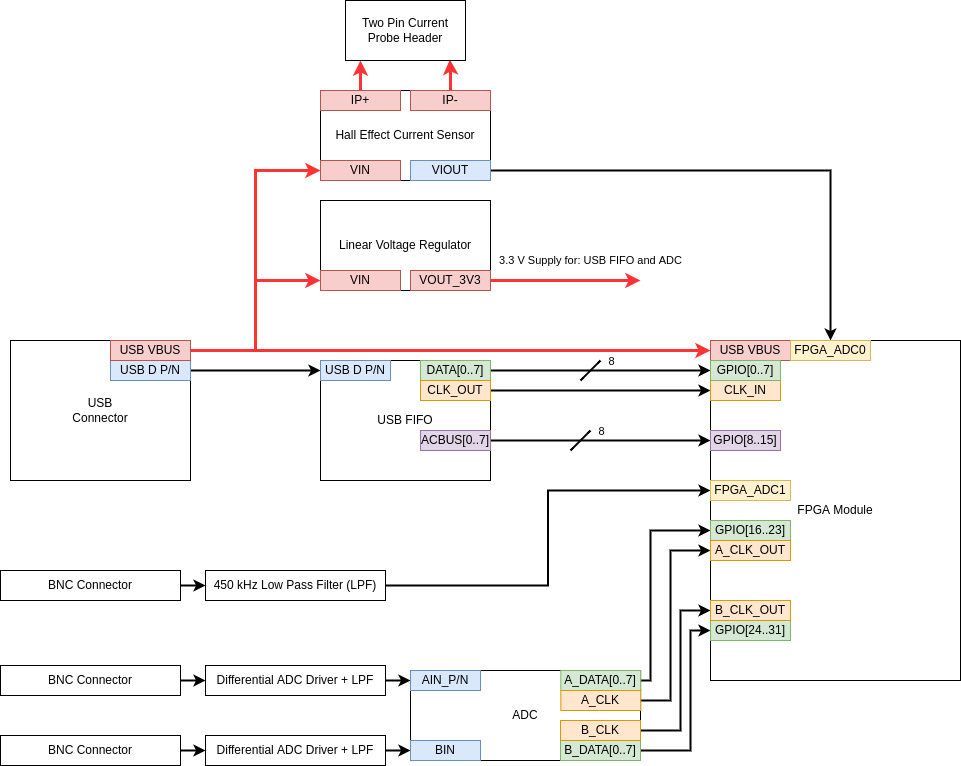
\includegraphics[width=16cm]{../../misc/TeachEE-System-Diagram.drawio.png}
            \caption{TeachEE PCB System Block Diagram}
            \label{fig:pcb-block-diagram}
        \end{figure}
        \begin{landscape}
        \section{Schematics}
        \label{appendix:schematic}
    \centering
    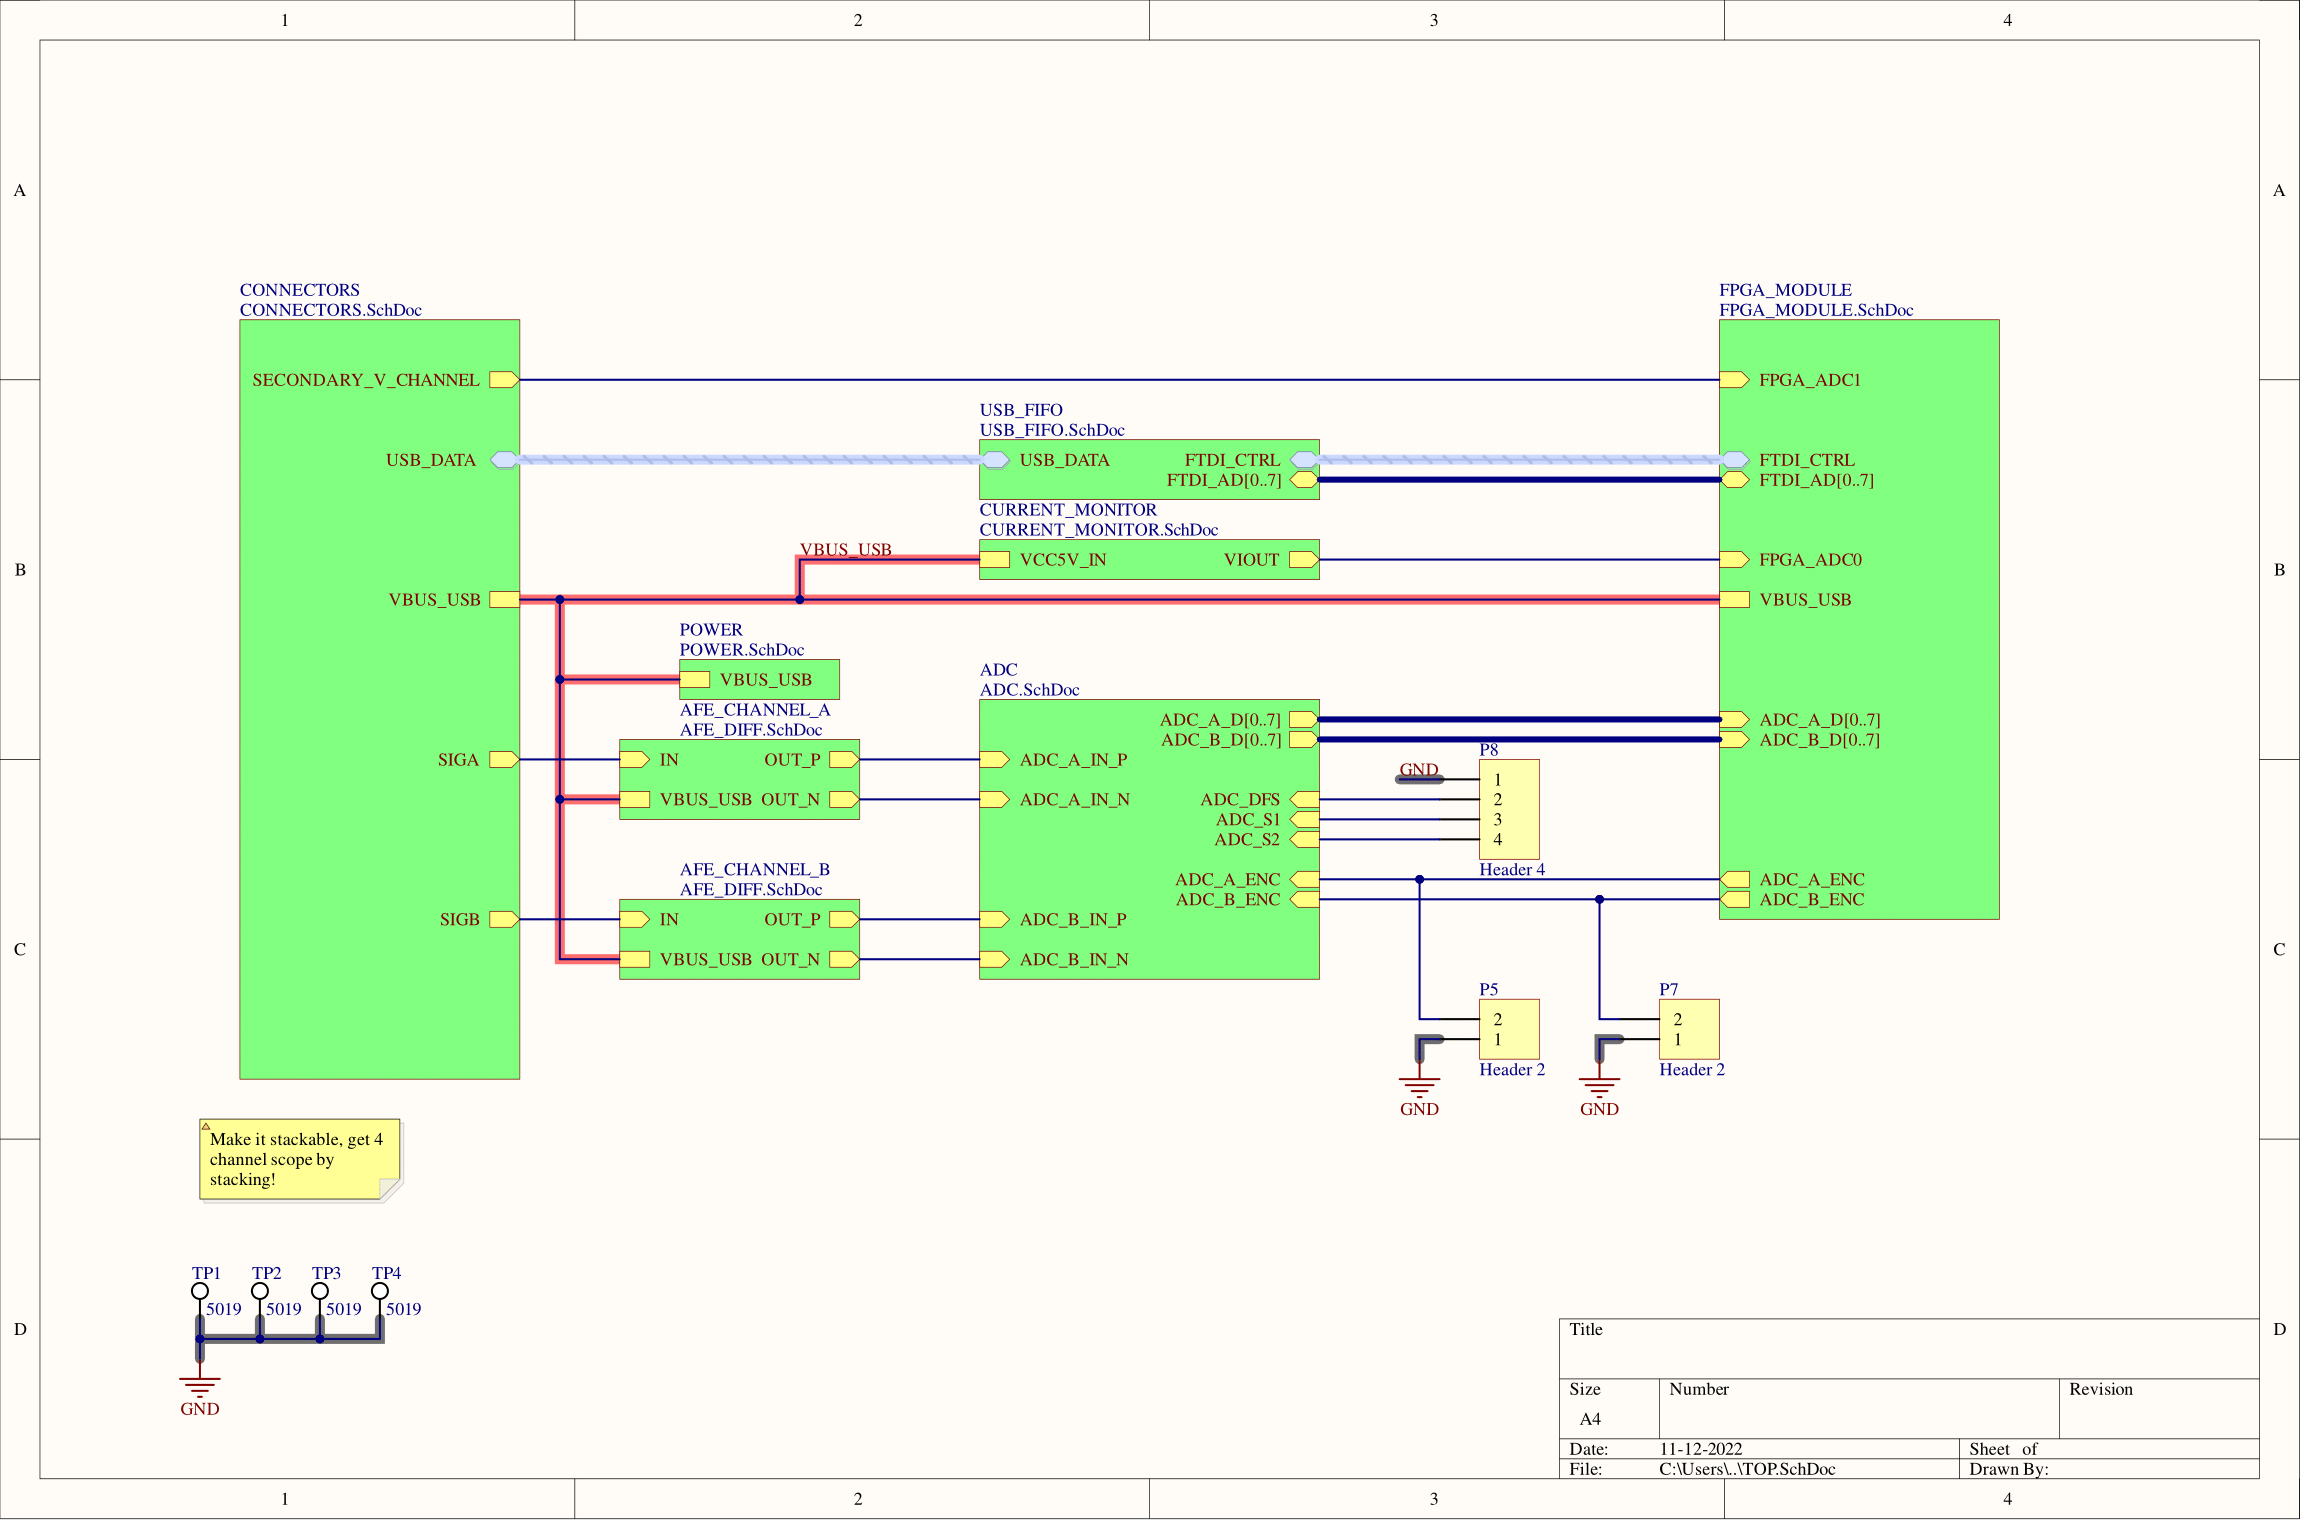
\includegraphics[height=15cm]{schematics/schematic1-1.png}
        \end{landscape}
    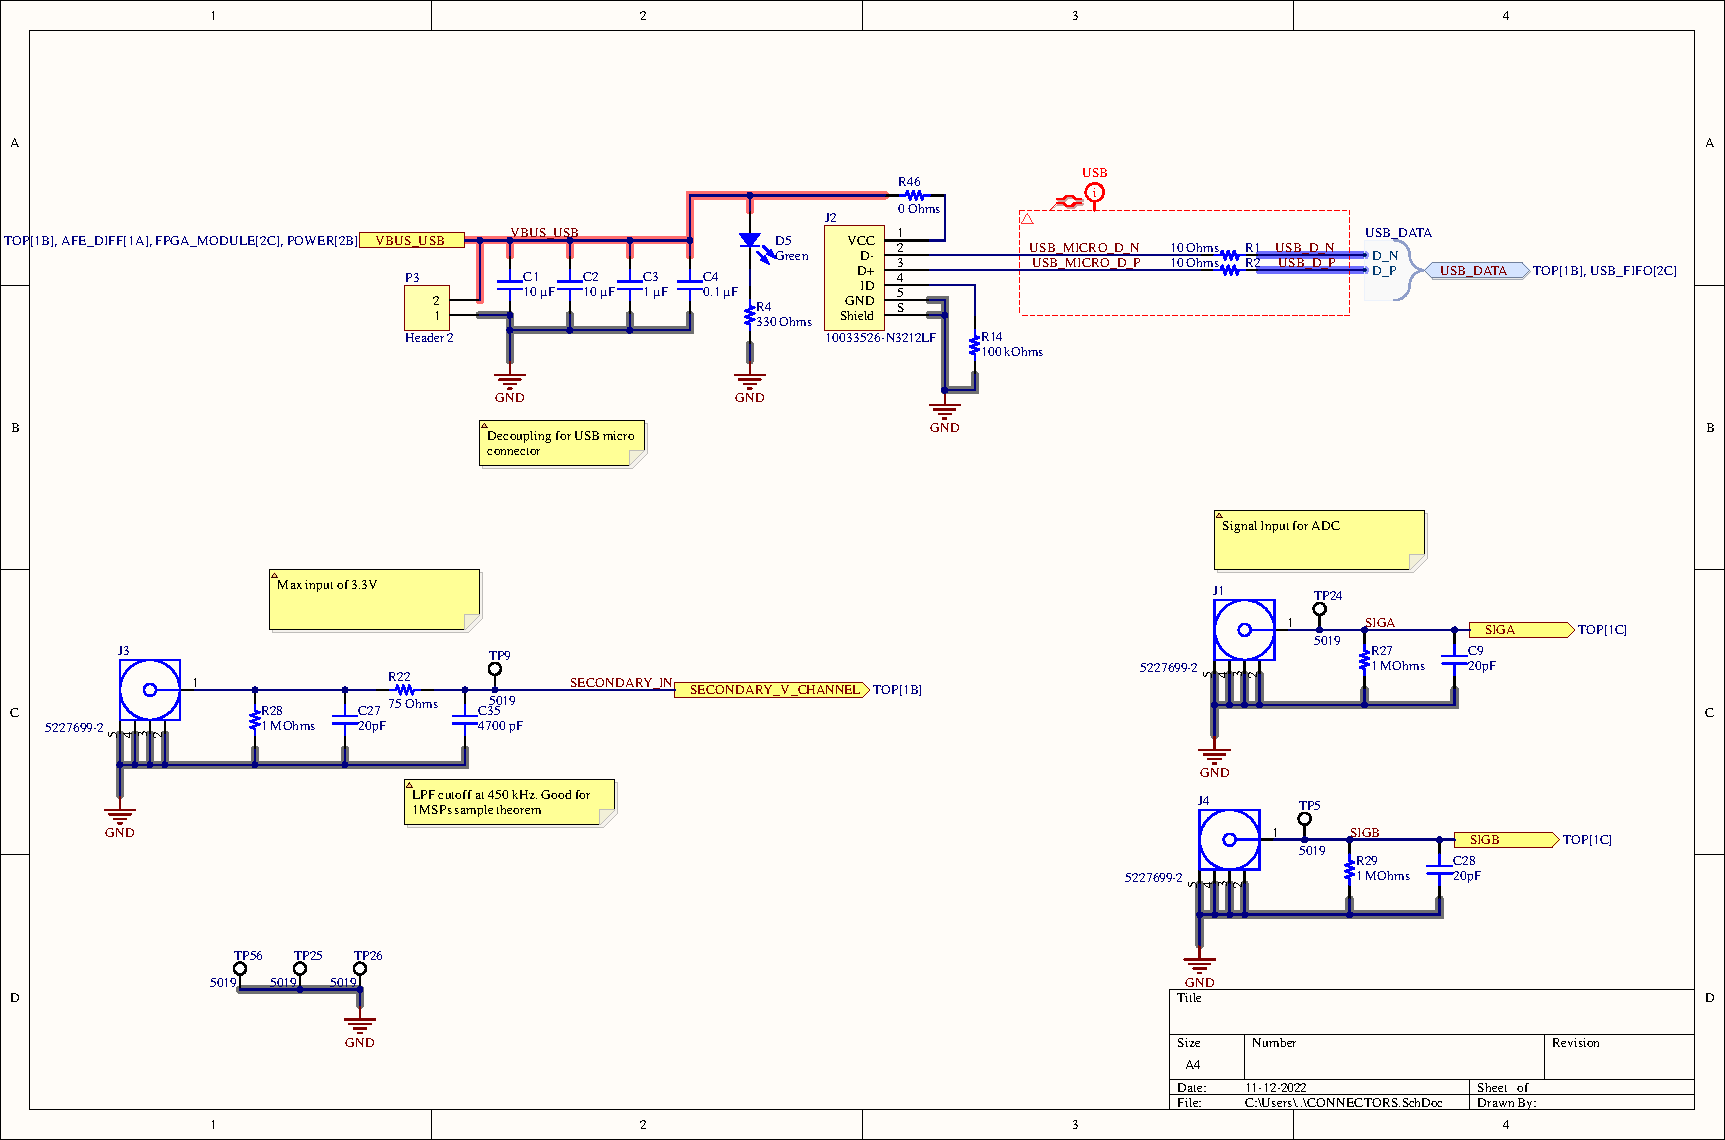
\includepdf[pages=-,landscape=true]{schematics/schematic2-8.pdf}

        \begin{landscape}
        \section{PCB Layout}
        \label{appendix:layout}
    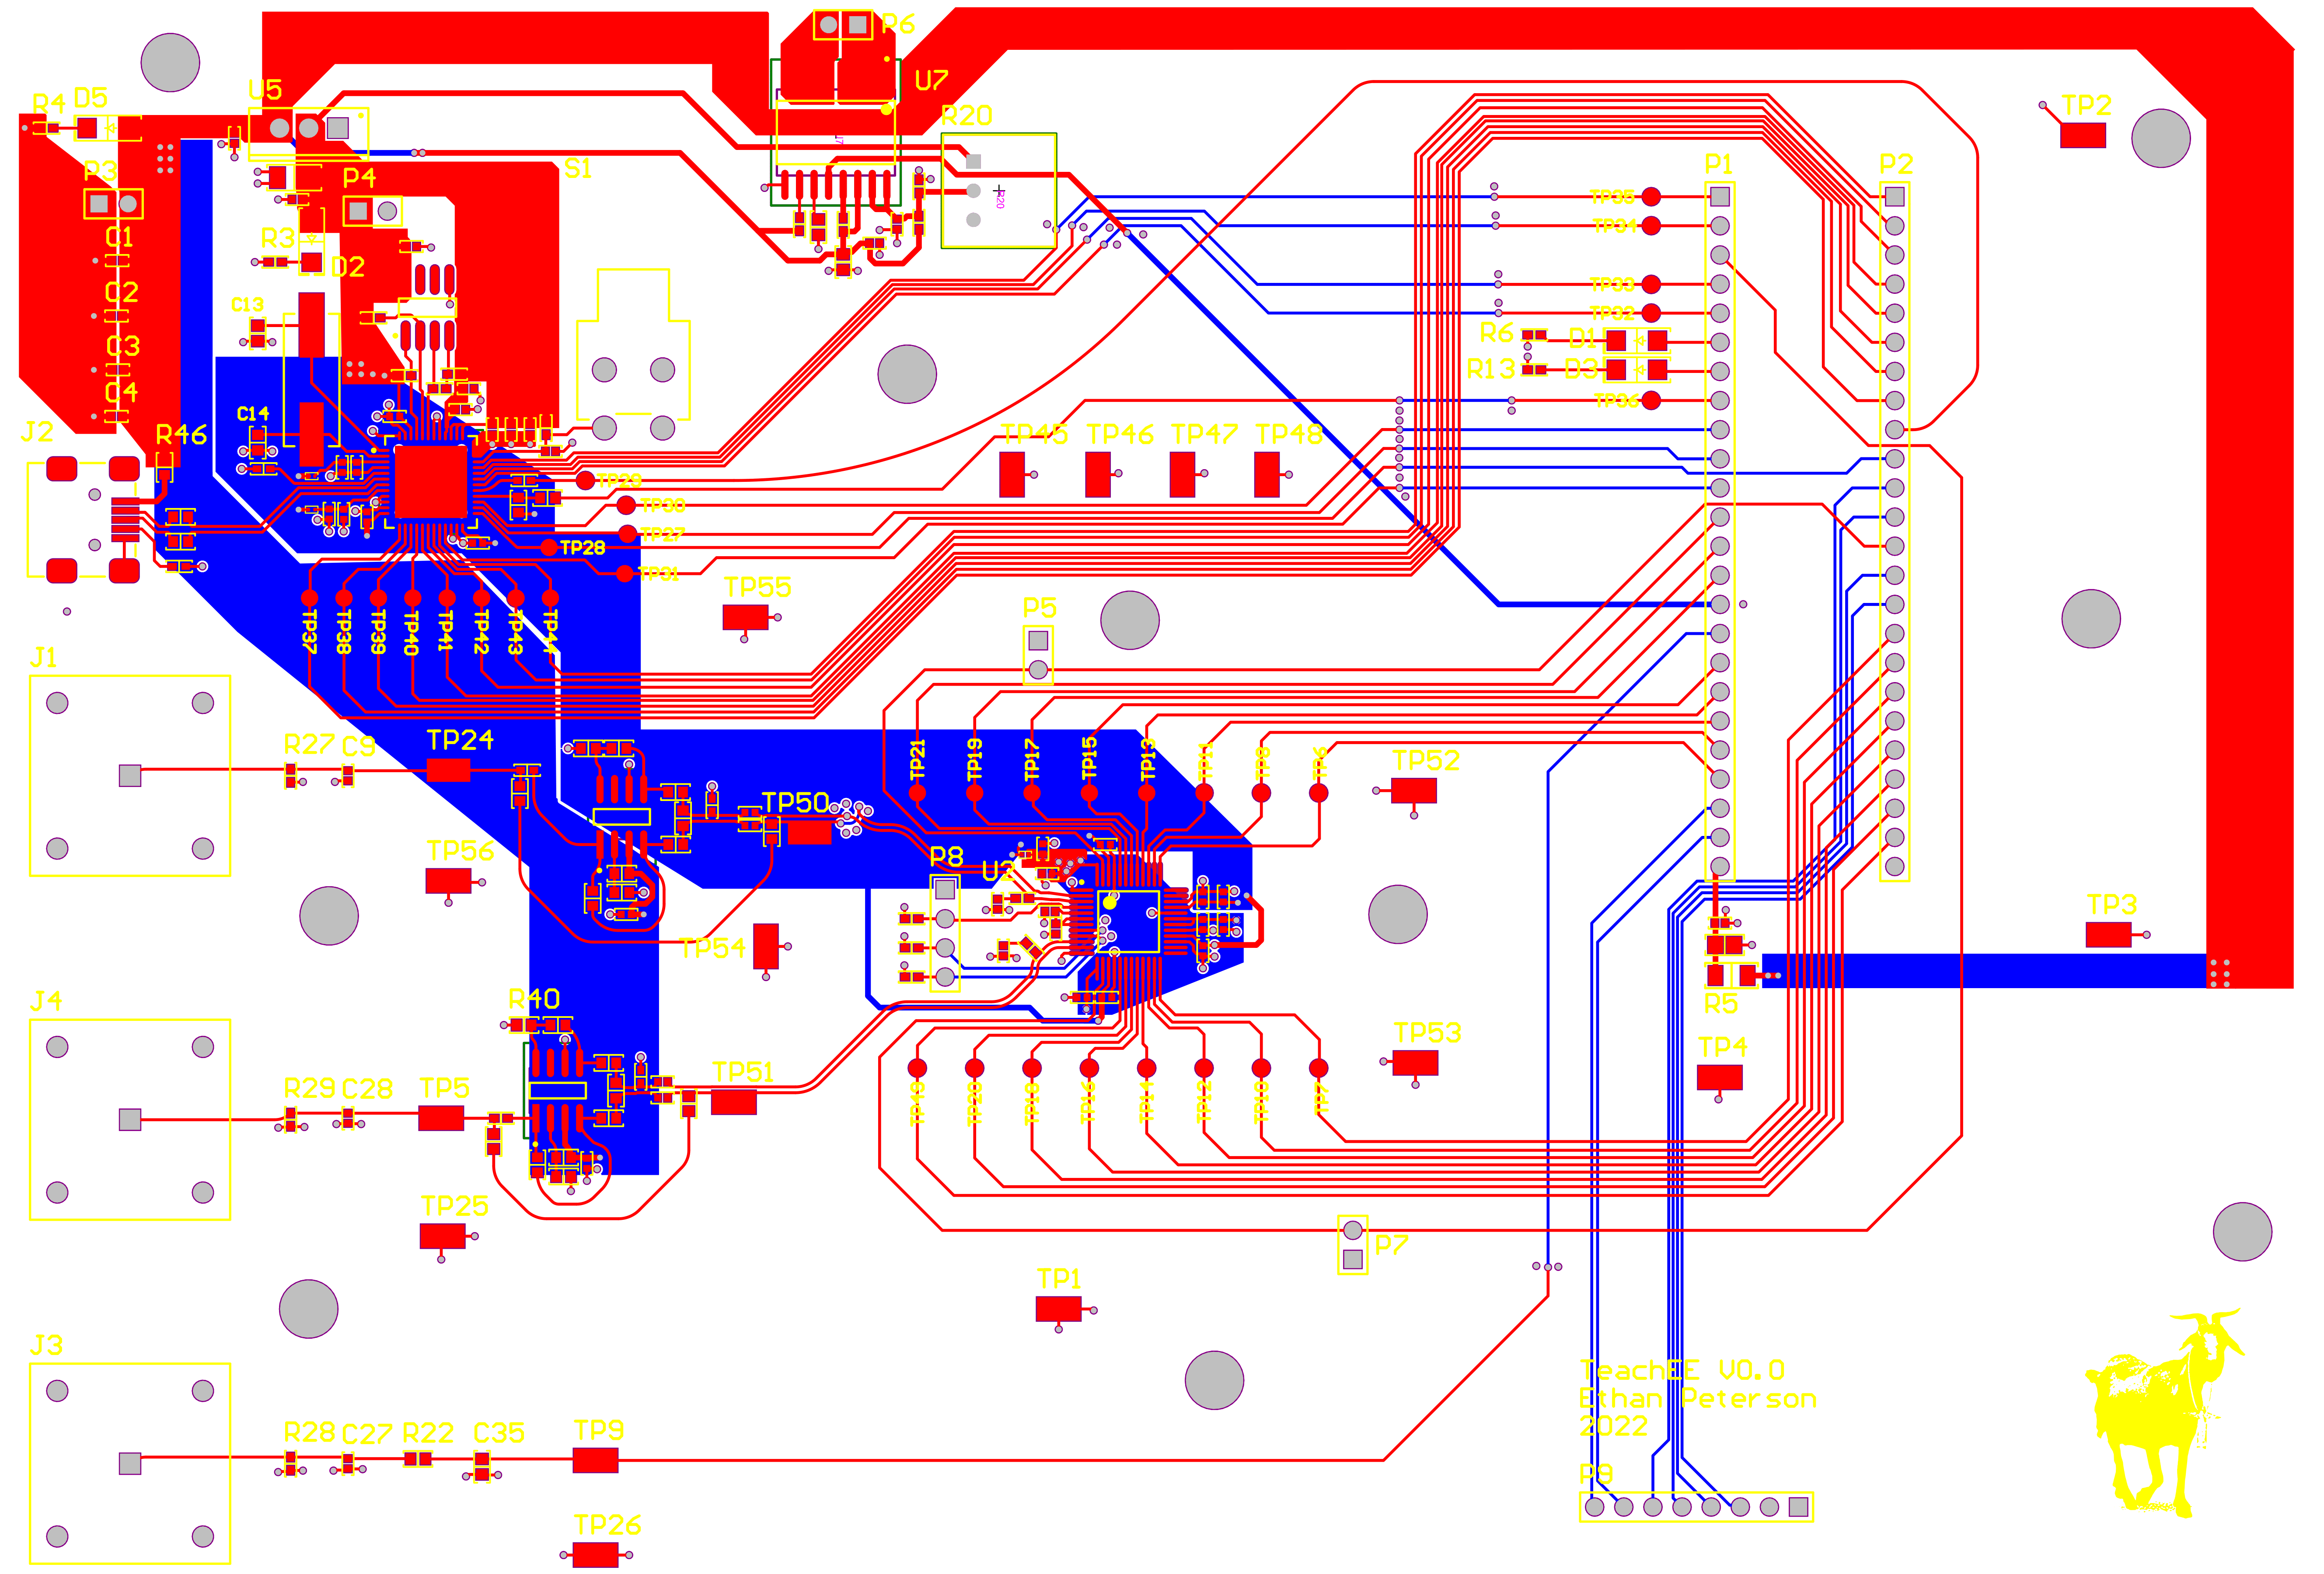
\includegraphics[height=15cm]{schematics/Layout.png}
        \end{landscape}

        \section{PCB Bill of Materials}
        \label{appendix:bom}
    \begin{table}[H]
    \begin{tabular}{p{1.7in}|p{0.3in}|p{0.8in}|p{0.7in}|p{0.7in}|p{1in}}
        \textbf{Designator} & \textbf{QTY} & \textbf{Description} & \textbf{Comment} & \textbf{Footprint} & \textbf{Part Number} \\ \hline 
        C1, C2, C37, C48 & 4 & CAP CER 10UF 10V X5R 0402 & 10 µF & CAP 0402\_1005 & CL05A106MP8NUB8 \\ \hline
        C3 & 1 & CAP CER 1UF 10V X7S 0402 & 1 µF & CAP 0402\_1005 & GRM155C71A105KE11D \\ \hline
        C4, C11, C16, C17, C18, C19, C20, C21, C22, C24, C26, C29, C30, C38, C39, C40, C41, C42, C43, C44, C45, C46, C47, C50\_AFE\_CHANNEL\_A, C50\_AFE\_CHANNEL\_B, C52\_AFE\_CHANNEL\_A, C52\_AFE\_CHANNEL\_B, C53\_AFE\_CHANNEL\_A, C53\_AFE\_CHANNEL\_B & 29 & CAP CER 0.1UF 50V X5R 0402 & 0.1 µF & CAP 0402\_1005 & CGA2B3X5R1H104M050BB \\ \hline
        C5, C12, C32, C34 & 4 & CAP CER 0.1UF 10V X7R 0402 & 0.1µF & CAP 0402\_1005 & 0402ZC104KAT2A \\ \hline
        C6 & 1 & CAP CER 10UF 16V X5R 1206 & 10 µF & CAP 1206\_3216 - 0.8MM & EMK316BJ106MD-T \\ \hline
        C7 & 1 & CAP CER 10UF 35V X6S 0805 & 10 µF & CAP 0805\_2012 & GRM21BC8YA106KE11L \\ \hline
        C8, C15, C23, C25 & 4 & CAP CER 4.7UF 16V X5R 0402 & 4.7 µF & CAP 0402\_1005 & CL05A475MO5NUNC \\ \hline
        C9, C27, C28 & 3 & CAP CER 20PF 25V NP0 0402 & 20pF & CAP 0402\_1005 & 04023U200JAT2A \\ \hline
    \end{tabular}
    \end{table}

    \newpage

    \begin{table}[H]
    \begin{tabular}{p{1.7in}|p{0.3in}|p{0.8in}|p{0.7in}|p{0.7in}|p{1in}}
        \textbf{Designator} & \textbf{QTY} & \textbf{Description} & \textbf{Comment} & \textbf{Footprint} & \textbf{Part Number} \\ \hline 
        C10 & 1 & CAP MLCC 0.01UF 100V X7R 0402 & 10000 pF & CAP 0402\_1005 & HMK105B7103KVHFE \\ \hline
        C13, C14 & 2 & CAP CER 36PF 100V NP0 0603 & 36pF & CAP 0603\_1608 & 06031A360JAT2A \\ \hline
        C31 & 1 & CAP CER 1UF 16V X7R 0603 & 1 µF & CAP 0603\_1608 & C0603C105K4RACAUTO \\ \hline
        C33, C35 & 2 & CAP CER 0603 4.7NF 16V X7R 10\% & 4700 pF & CAP 0603\_1608 & C0603C472K4RECAUTO \\ \hline
        C51\_AFE\_CHANNEL\_A, C51\_AFE\_CHANNEL\_B & 2 & CAP CER 15PF 25V C0G/NP0 0603 & 15 pF & CAP 0603\_1608 & C0603C150J3GACAUTO \\ \hline
        D1, D3 & 2 & LED SMD & Blue & LED 1206\_3216 BLUE & APTL3216QBC/D-01 \\ \hline
        D2, D5 & 2 & LED SMD & Green & LED 1206\_3216 GREEN & APTL3216ZGCK-01 \\ \hline
        FB1, FB2, FB3 & 3 & FERRITE BEAD 33 OHM 0201 1LN & 33 Ohms @ 100 MHz & FER 0201\_0603 & MMZ0603F330CT000 \\ \hline
        J1, J3, J4 & 3 & Jack BNC Connector, 1 Position, Height 16.26 mm, Tail Length 6.35 mm, -55 to 85 degC, RoHS, Tube & 5227699-2 & & 5227699-2 \\ \hline
        J2 & 1 & CONN RCPT MINI USB B 5POS SMD RA & & & 10033526-N3212LF \\ \hline
    \end{tabular}
    \end{table}
    \newpage
    \begin{table}[H]
        \begin{tabular}{p{1.7in}|p{0.3in}|p{0.8in}|p{0.7in}|p{0.7in}|p{1in}}
        \textbf{Designator} & \textbf{QTY} & \textbf{Description} & \textbf{Comment} & \textbf{Footprint} & \textbf{Part Number} \\ \hline 
        R1, R2 & 2 & RES SMD 10 OHM 0.1\% 1/10W 0603 & 10 Ohms & RES 0603\_1608 & CRT0603-BY-10R0ELF \\ \hline
        R3, R6, R13 & 3 & RES 220 OHM 1\% 1/8W 0402 & 220 Ohms & RES 0402\_1005 & CRGP0402F220R \\ \hline
        R4 & 1 & RES SMD 330 OHM 5\% 1/16W 0402 & 330 Ohms & RES 0402\_1005 & AC0402JR-07330RL \\ \hline
        R5 & 1 & 1206 40 AMP JUMPER & 0 Ohms & RES 1206\_3216 & JR1206X40E \\ \hline
        R7 & 1 & RES SMD 12K OHM 0.1\% 1/16W 0402 & 12 kOhms & RES 0402\_1005 & CPF0402B12KE1 \\ \hline
        R8, R9, R10, R11, R17, R18, R19, R21, R32, R33, R34 & 11 & RES 10K OHM 0.1\% 1/10W 0402 & 10 kOhms & RES 0402\_1005 & RP73PF1E10KBTD \\ \hline
        R12 & 1 & RES 1.8K OHM 1\% 1/16W 0402 & 1.8 kOhms & RES 0402\_1005 & RC0402FR-071K8L \\ \hline
        R14 & 1 & RES SMD 100K OHM 0.1\% 1/16W 0402 & 100 kOhms & RES 0402\_1005 & CPF0402B100KE \\ \hline
        R15, R46 & 2 & RES SMD 0 OHM JUMPER 1/2W 0603 & 0 Ohms & RES 0603\_1608 & 5110 \\ \hline
        R22 & 1 & RES SMD 75 OHM 1\% 1/10W 0603 & 75 Ohms & RES 0603\_1608 & AC0603FR-0775RL \\ \hline
        R26 & 1 & RES 24 OHM 1\% 1/16W 0402 & 24 Ohms & RES 0402\_1005 & RC0402FR-0724RL \\ \hline
        \end{tabular}
    \end{table}
    \newpage
    \begin{table}[H]
        \begin{tabular}{p{1.7in}|p{0.3in}|p{0.8in}|p{0.7in}|p{0.7in}|p{1in}}
        \textbf{Designator} & \textbf{QTY} & \textbf{Description} & \textbf{Comment} & \textbf{Footprint} & \textbf{Part Number} \\ \hline 
        R27, R28, R29 & 3 & RES 1M OHM 1\% 1/16W 0402 & 1 MOhms & RES 0402\_1005 & RMCF0402FT1M00 \\ \hline
        R36\_AFE\_CHANNEL\_A, R36\_AFE\_CHANNEL\_B & 2 & RES SMD 523 OHM 0.1\% 1/16W 0402 & 523 Ohms & RES 0402\_1005 & ERA-2ARB5230X \\ \hline
        R37\_AFE\_CHANNEL\_A, R37\_AFE\_CHANNEL\_B, R40\_AFE\_CHANNEL\_A, R40\_AFE\_CHANNEL\_B, R41\_AFE\_CHANNEL\_A, R41\_AFE\_CHANNEL\_B & 6 & RES SMD 500 OHM 0.05\% 1/10W 0603 & 500 Ohms & RES 0603\_1608 & TNPU0603500RAZEN00 \\ \hline
        R39\_AFE\_CHANNEL\_A, R39\_AFE\_CHANNEL\_B, R43\_AFE\_CHANNEL\_A, R43\_AFE\_CHANNEL\_B & 4 & RES 50 OHM 5\% 1/8W 0603 & 50 Ohms & RES 0603\_1608 & CH0603-50RJNTA \\ \hline
        R42\_AFE\_CHANNEL\_A, R42\_AFE\_CHANNEL\_B & 2 & RES SMD 4.02K OHM 1\% 1/10W 0603 & 4.02 kOhms & RES 0603\_1608 & AC0603FR-074K02L \\ \hline
        R44\_AFE\_CHANNEL\_A, R44\_AFE\_CHANNEL\_B & 2 & RES SMD 1K OHM 1\% 1/10W 0603 & 1 kOhms & RES 0603\_1608 & AA0603FR-071KL \\ \hline
        R45\_AFE\_CHANNEL\_A, R45\_AFE\_CHANNEL\_B & 2 & RES 25 OHM 0.1\% 1/20W 0402 & 25 Ohms & RES 0402\_1005 & FC0402E25R0BST0 \\ \hline
        S1 & 1 & SWITCH PUSH SPST-NO 0.4VA 28V & &  & AB11AH-HA \\ \hline
        TP1, TP2, TP3, TP4, TP5, TP9, TP24, TP25, TP26, TP45, TP46, TP47, TP48, TP50, TP51, TP52, TP53, TP54, TP55, TP56 & 20 & Test Point, 1 Position SMD, RoHS, Tape and Reel & 5019 & KSTN5019 & 5019 \\ \hline
        U1 & 1 & IC HS USB TO UART/FIFO 48QFN & FT232 & QFN-48 & FT232HQ-REEL \\ \hline
        \end{tabular}
    \end{table}
    \newpage
    \begin{table}[H]
        \begin{tabular}{p{1.7in}|p{0.3in}|p{0.8in}|p{0.7in}|p{0.7in}|p{1in}}
        \textbf{Designator} & \textbf{QTY} & \textbf{Description} & \textbf{Comment} & \textbf{Footprint} & \textbf{Part Number} \\ \hline 
        U2 & 1 & Dual 8-Bit AD Converter with Parallel Interface, 40MSPS, -40 to +85 degC, ST-48, Pb-Free, Tray &  & ST-48M & AD9288BSTZ-40 \\ \hline
        U3\_AFE\_CHANNEL\_A, U3\_AFE\_CHANNEL\_B & 2 & IC ADC DRIVER 8SOIC & AD8138 & R-8-IPC\_A & AD8138ARZ-R7 \\ \hline
        U5 & 1 & Fixed Low Drop Positive Voltage Regulator, 3.3V, 3-Pin TO-220 & LD1117 & TO220 & LD1117V33C \\ \hline
        U6 & 1 & 2K, 128x16-bit, 2.5V Microwire Serial EEPROM, 8-Pin SOIC 150mil, Commercial Temperature, Tape and Reel & 93LC56 & SOIC8 & 93LC56BT/SN \\ \hline
        U7 & 1 & CURRENT SENSOR & ACS720 &  & ACS720KLATR-15AB-T \\ \hline
        Y1 & 1 & CRYSTAL 12.0000MHZ 20PF SMD & 12 MHz & ABLS & ABLS-12.000MHZ-20-B-3-H-T \\ \hline
        \end{tabular}
    \end{table}

        \section{TeachEE Desktop App Screenshots}
    \begin{figure}[H]
        \centering
        % 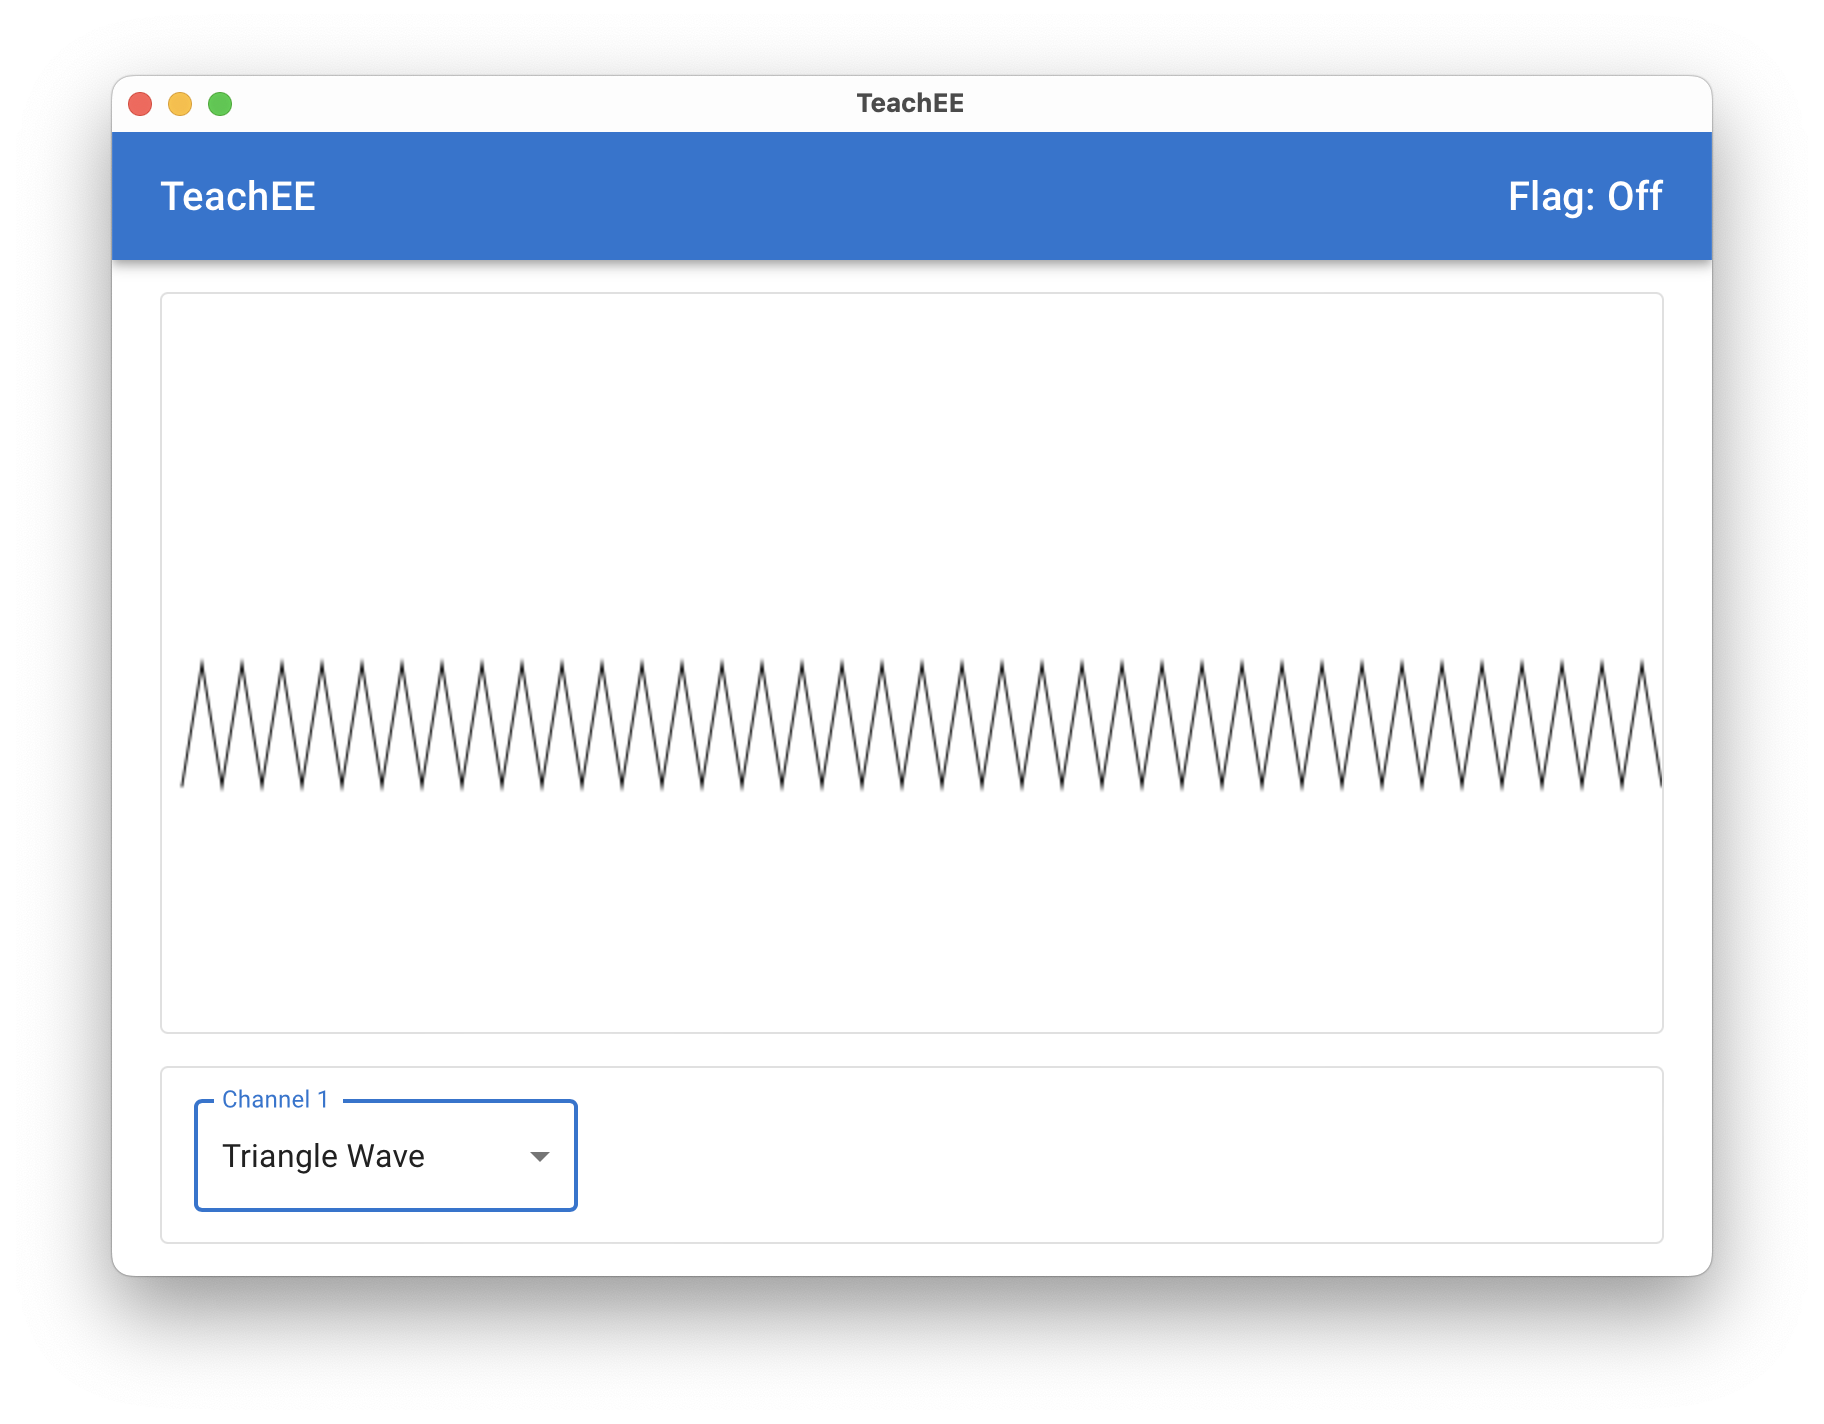
\includegraphics[width=\textwidth]{./schematics/sw-screenshot.png}
        \caption{TeachEE Desktop App Displaying a Triangle Wave}
    \end{figure}
    \end{appendices}
\end{document}
